\documentclass[10pt,letterpaper]{article}
\usepackage[utf8]{inputenc}
\usepackage{graphicx}
\usepackage{float}
\usepackage{epstopdf}

\begin{document}
\begin{center}
CMPE245 Project 2
\end{center}
Chien-Pin Chen\\
06/07/2016\\

\noindent \textbf{Part 1} Design my extended Kalman filter (EKF):\\
In Extended Kalman Filter, equation 1, 2, and 3 of the project 2 could rewrite to a full system model as:
\begin{equation}
	\frac{d}{{dt}}\left[ {\begin{array}{*{20}c}
	   x  \\
	   y  \\
	   z  \\
	   {\dot x}  \\
	   {\dot y}  \\
	   {\dot z}  \\
	   \psi   \\
	\end{array}} \right] = \left[ {\begin{array}{*{20}c}
	   {\dot x}  \\
	   {\dot y}  \\
	   {\dot z}  \\
	   {\{ c\}  \cdot g(\sin \psi \sin \varphi  + \cos \psi \cos \varphi \sin \theta )}  \\
	   {\{ c\}  \cdot g(\sin \psi \cos \varphi \sin \theta  - \cos \psi \sin \varphi )}  \\
	   {\{ c\}  \cdot (g\cos \varphi \cos \theta  - g)}  \\
	   0  \\
	\end{array}} \right] + \left[ {\begin{array}{*{20}c}
	   {0_{3 \times 4} }  \\
	   {\begin{array}{*{20}c}
	   {\delta _x } & 0 & 0 & 0  \\
	   0 & {\delta _y } & 0 & 0  \\
	   0 & 0 & {\delta _z } & 0  \\
	   0 & 0 & 0 & {\delta _\psi  }  \\
	\end{array}}  \\
	\end{array}} \right]\left[ {\begin{array}{*{20}c}
	   {\xi _x }  \\
	   {\xi _y }  \\
	   {\xi _z }  \\
	   {\xi _\psi  }  \\
	\end{array}} \right]
\end{equation}

And, equation 1 could be refer to:
\begin{equation}
	\begin{array}{l}
	 dx = xdt + \delta dw \\ 
	 X_{k + 1}  = X_k  + X_k \Delta t + \delta \sqrt {\Delta t} W \\ 
	 \end{array}
\end{equation}
Then, for computing, I could set:
\begin{eqnarray}
	\begin{array}{l}
	 x_{k + 1}  = f_k (\hat x_k ,0) \\ 
	 x_{k + 1}  = \left[ {\begin{array}{*{20}c}
	   {x_1 (k + 1)}  \\
	   {x_2 (k + 1)}  \\
	   {x_3 (k + 1)}  \\
	   \begin{array}{l}
	 x_4 (k + 1) \\ 
	 x_5 (k + 1) \\ 
	 x_6 (k + 1) \\ 
	 x_7 (k + 1) \\ 
	 \end{array}  \\
	\end{array}} \right] = \left[ {\begin{array}{*{20}c}
	   {x_1 (k) + \Delta t \cdot x_4 }  \\
	   {x_2 (k) + \Delta t \cdot x_5 }  \\
	   {x_3 (k) + \Delta t \cdot x_6 }  \\
	   \begin{array}{l}
	 x_4 (k) + \Delta t \cdot \{ c\}  \cdot g(\sin x_7 \sin \varphi  + \cos x_7 \cos \varphi \sin \theta ) \\ 
	 x_5 (k) + \Delta t \cdot \{ c\}  \cdot g(\sin x_7 \cos \varphi \sin \theta  - \cos x_7 \sin \varphi ) \\ 
	 x_6 (k) + \Delta t \cdot \{ c\}  \cdot (g\cos \varphi \cos \theta  - g) \\ 
	 x_7 (k) \\ 
	 \end{array}  \\
	\end{array}} \right] \\ 
	 \end{array}\\
	\Phi _k  = \frac{{\partial f_k (\hat x_k ,0)}}{{\partial x_k }} = \left[ {\begin{array}{*{20}c}
	   1 & 0 & 0 & {\Delta t} & 0 & 0 & 0  \\
	   0 & 1 & 0 & 0 & {\Delta t} & 0 & 0  \\
	   0 & 0 & 1 & 0 & 0 & {\Delta t} & 0  \\
	   0 & 0 & 0 & 1 & 0 & 0 & {\Delta t \cdot \{ c\}  \cdot g(\cos x_7 \sin \varphi  + \sin x_7 \cos \varphi \sin \theta )}  \\
	   0 & 0 & 0 & 0 & 1 & 0 & {\Delta t \cdot \{ c\}  \cdot g(\cos x_7 \cos \varphi \sin \theta  + \sin x_7 \sin \varphi )}  \\
	   0 & 0 & 0 & 0 & 0 & 1 & 0  \\
	   0 & 0 & 0 & 0 & 0 & 0 & 1  \\
	\end{array}} \right]\\
	\Gamma _k  = \frac{{\partial f_k (\hat x_k ,0)}}{{\partial w_k }} = \left[ {\begin{array}{*{20}c}
	   {0_{3 \times 4} }  \\
	   {\begin{array}{*{20}c}
	   {\delta _x \sqrt {dt} } & 0 & 0 & 0  \\
	   0 & {\delta _y \sqrt {dt} } & 0 & 0  \\
	   0 & 0 & {\delta _z \sqrt {dt} } & 0  \\
	   0 & 0 & 0 & {\delta _\psi  \sqrt {dt} }  \\
	\end{array}}  \\
	\end{array}} \right]
	Q = \left[ {\begin{array}{*{20}c}
	   1 & 0 & 0 & 0  \\
	   0 & 1 & 0 & 0  \\
	   0 & 0 & 1 & 0  \\
	   0 & 0 & 0 & 1  \\
	\end{array}} \right]
\end{eqnarray}
In equation (3), (4), and (5), $\Delta t$ and $dt$ are non-constant sampling time which are assigned by 
dtrec in data3D.mat. Also, in equation (1), because $\xi_x(t)$, $\xi_y(t)$, $\xi_z(t)$ and $\xi_\psi(t)$ are 
zero-mean white noises, I set $\delta_x$, $\delta_y$, $\delta_z$ and $\delta_\psi$ as one at first. I will tune 
those intensity of process noise according to the result of extended Kalman filter later. In addition, the 
parameter $g$ is the gravitational acceleration (constant, as $9.81 kgm/s^2$), and the parameter $c$ is 
also a constant (set to $1$) in part 1 of project 2.
Next, the measurement model (equation (4) and (5)) of project 2 could refer to: 
\begin{equation}
	\underline{y}_k=\underline{h}_k(\underline{x}_k)+\underline{v}_k
\end{equation}
then, for computing EKF, I could set:
\begin{equation}
	{\rm H}_k  = \frac{{\partial h_k (\hat x_k ,0)}}{{\partial x_k }} = \left[ {\begin{array}{*{20}c}
	   1 & 0 & 0 & 0 & 0 & 0 & 0  \\
	   0 & 1 & 0 & 0 & 0 & 0 & 0  \\
	   0 & 0 & 1 & 0 & 0 & 0 & 0  \\
	   0 & 0 & 0 & 0 & 0 & 0 & 1  \\
	\end{array}} \right]
\end{equation}
\begin{equation}
	R = \left[ {\begin{array}{*{20}c}
	   {{\mathop{\rm var}} \{ x_m \} } & 0 & 0 & 0  \\
	   0 & {{\mathop{\rm var}} \{ y_m \} } & 0 & 0  \\
	   0 & 0 & {{\mathop{\rm var}} \{ z_m \} } & 0  \\
	   0 & 0 & 0 & {{\mathop{\rm var}} \{ \psi _m \} }  \\
	\end{array}} \right]
\end{equation}
In equation (8), $var\{x\}$, $var\{y\}$, and $var\{z\}$ are the variance of the measurement position and yaw 
angle of quad-rotor, and the measured noise of the Vicon is 10 cm. Therefore, I set $var\{x\}$, $var\{y\}$, and 
$var\{z\}$ as $0.1^2$ for initialization. Also, in the provided video, the yaw angle of the quad-rotor did not 
change a lot, so I set $var\{\psi\}=10\frac{\pi}{180}$ for initialization.\\
In the prediction step of Extended Kalman filter (EKF), I use following equations for discrete time model:
\begin{eqnarray}
	\underline{\hat{x}}_{k + 1}(-)  = \underline{\hat{f}}_k (\underline{\hat{x}}_k ,0)\\
	\underline{P}_{k + 1} ( - ) = \underline{\Phi}_k \underline{P}_k \underline{\Phi}_k^T + \underline{\Gamma}_k Q \underline{\Gamma}_k^T 
\end{eqnarray}
For initial guess of $\underline{\hat{x}}_0(-)$, I use the first element of the measurement data as $E\{x(0)\}$, 
$E\{y(0)\}$, $E\{z(0)\}$, and $E\{yaw(0)\}$, and I also use the second element with first to compute initial velocity 
 $E\{\dot{x}(0)\}$, $E\{\dot{y}(0)\}$, and $E\{\dot{z}(0)\}$:
\begin{equation}
	x_0  = \left[ {\begin{array}{*{20}c}
	   {x_m (0)}  \\
	   \begin{array}{l}
	 y_m (0) \\ 
	 z_m (0) \\ 
	 \end{array}  \\
	   \begin{array}{l}
	 {\raise0.7ex\hbox{${x_m (1) - x_m (0)}$} \!\mathord{\left/
	 {\vphantom {{x_m (1) - x_m (0)} {\Delta t}}}\right.\kern-\nulldelimiterspace}
	\!\lower0.7ex\hbox{${\Delta t}$}} \\ 
	 {\raise0.7ex\hbox{${y_m (1) - y_m (0)}$} \!\mathord{\left/
	 {\vphantom {{y_m (1) - y_m (0)} {\Delta t}}}\right.\kern-\nulldelimiterspace}
	\!\lower0.7ex\hbox{${\Delta t}$}} \\ 
	 {\raise0.7ex\hbox{${z_m (1) - z_m (0)}$} \!\mathord{\left/
	 {\vphantom {{z_m (1) - z_m (0)} {\Delta t}}}\right.\kern-\nulldelimiterspace}
	\!\lower0.7ex\hbox{${\Delta t}$}} \\ 
	 \end{array}  \\
	   {yaw_m (0)}  \\
	\end{array}} \right]
\end{equation} 
For my initial guess of $\underline{\hat{P}}_0$, I use the variance of the measurement noise as initial values 
for the variance of process noise of the position (x, y, z, and yaw). Also, my initial expected velocity is acquired 
from initial position of quad-rotor, so I set the covariance of $\dot{x}_0$, $\dot{y}_0$, $\dot{z}_0$ according to 
the variance of the position. The following is how I initialize the state covariance matrix:
\begin{equation}
	\begin{array}{l}
	 {\mathop{\rm cov}} \{ x,x\}  = P_{11}  = P_{22}  = P_{33}  = measure\_noise^2  \\ 
	 {\mathop{\rm cov}} \{ \dot x,\dot x\}  = P_{44}  = P_{55}  = P_{66}  = 2P_{11} /\Delta t^2  \\ 
	 {\mathop{\rm cov}} \{ \theta ,\theta \}  = P_{77}  = (10{\raise0.7ex\hbox{${pi}$} \!\mathord{\left/
	 {\vphantom {{pi} {180}}}\right.\kern-\nulldelimiterspace}
	\!\lower0.7ex\hbox{${180}$}})^2  \\ 
	 P_{14}  = P_{25}  = P_{36}  = P_{11}  \\ 
	 P_{12}  = P_{13}  = P_{23}  = P_{45}  = P_{46}  = P_{56}  = 0 \\ 
	 P_0  = \left[ {\begin{array}{*{20}c}
	   {P_{11} } & 0 & 0 & {P_{14} } & 0 & 0 & 0  \\
	   0 & {P_{22} } & 0 & 0 & {P_{25} } & 0 & 0  \\
	   0 & 0 & {P_{33} } & 0 & 0 & {P_{36} } & 0  \\
	   {P_{14} } & 0 & 0 & {P_{44} } & 0 & 0 & 0  \\
	   0 & {P_{25} } & 0 & 0 & {P_{55} } & 0 & 0  \\
	   0 & 0 & {P_{36} } & 0 & 0 & {P_{66} } & 0  \\
	   0 & 0 & 0 & 0 & 0 & 0 & {P_{77} }  \\
	\end{array}} \right] \\ 
	 \end{array}
\end{equation}
Next, I use following equations in the update step of EKF:
\begin{eqnarray}
	\underline{K}_{k + 1}  = \underline{P}_{k + 1} ( - )\underline{H}_{k + 1}^T (\underline{H}_{k + 1} \underline{P}_{k+ 1} ( - )\underline{H}_{k + 1}^T  + \underline{R}_{k + 1} )^{ - 1} \\
	\underline{\hat{x}}_{k + 1}  = \underline{\hat{x}}_{k + 1} ( - ) + \underline{K}_{k + 1} (\underline{y}_{k + 1}  - \underline{h}_{k + 1} (\underline{\hat{x}}_{k + 1} ( - )))\\
	\underline{P}_{k + 1}  = (I - \underline{K}_{k + 1} \underline{H}_{k + 1} )\underline{P}_{k + 1} ( - )
\end{eqnarray}
After updating, do another extended Kalman filter with next measurement data $y(k)$, which is provided in 
data3d.mat file. In order to let the result of prediction to fit with the measure data (such as let the changing of 
x,y, and z to have the similar scale as the changing in the measurement data), I modify some values in the 
covariance matrices of the process and measured noise, as in figure 1 and figure 2. From the result of figure 
1 ( 3D position), the predicted position is not fit with the measurement data, but the result of figure 2 shows 
that the predicted position (x, y, and z) did not diverge from the measurement data. Also, from the result of 
figure 2, the expected yaw ($\psi$) angle is more stable than the measurement yaw angle.
 \begin{figure}[H]
	 \begin{center}
	 	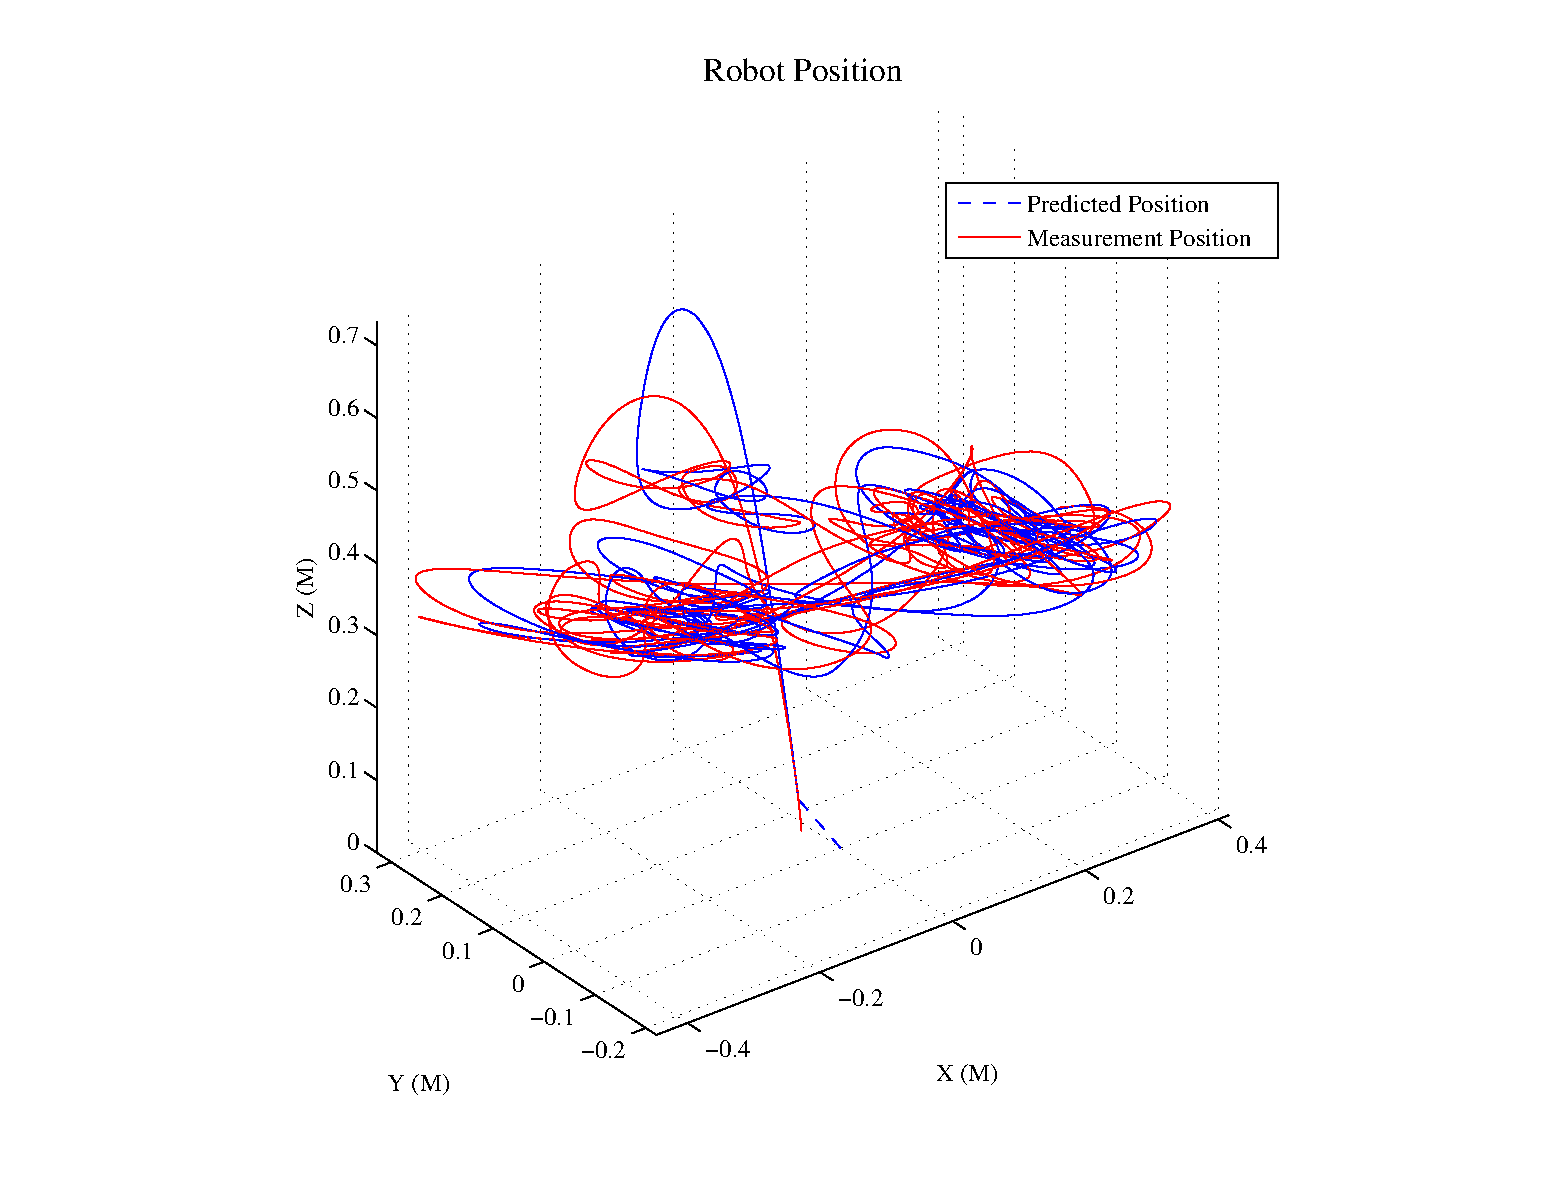
\includegraphics[width=\textwidth]{part1_3d.eps}
	 	\caption{The result of Robot Position in 3D space.}
	 \end{center}
 \end{figure}
  \begin{figure}[H]
	 \begin{center}
	 	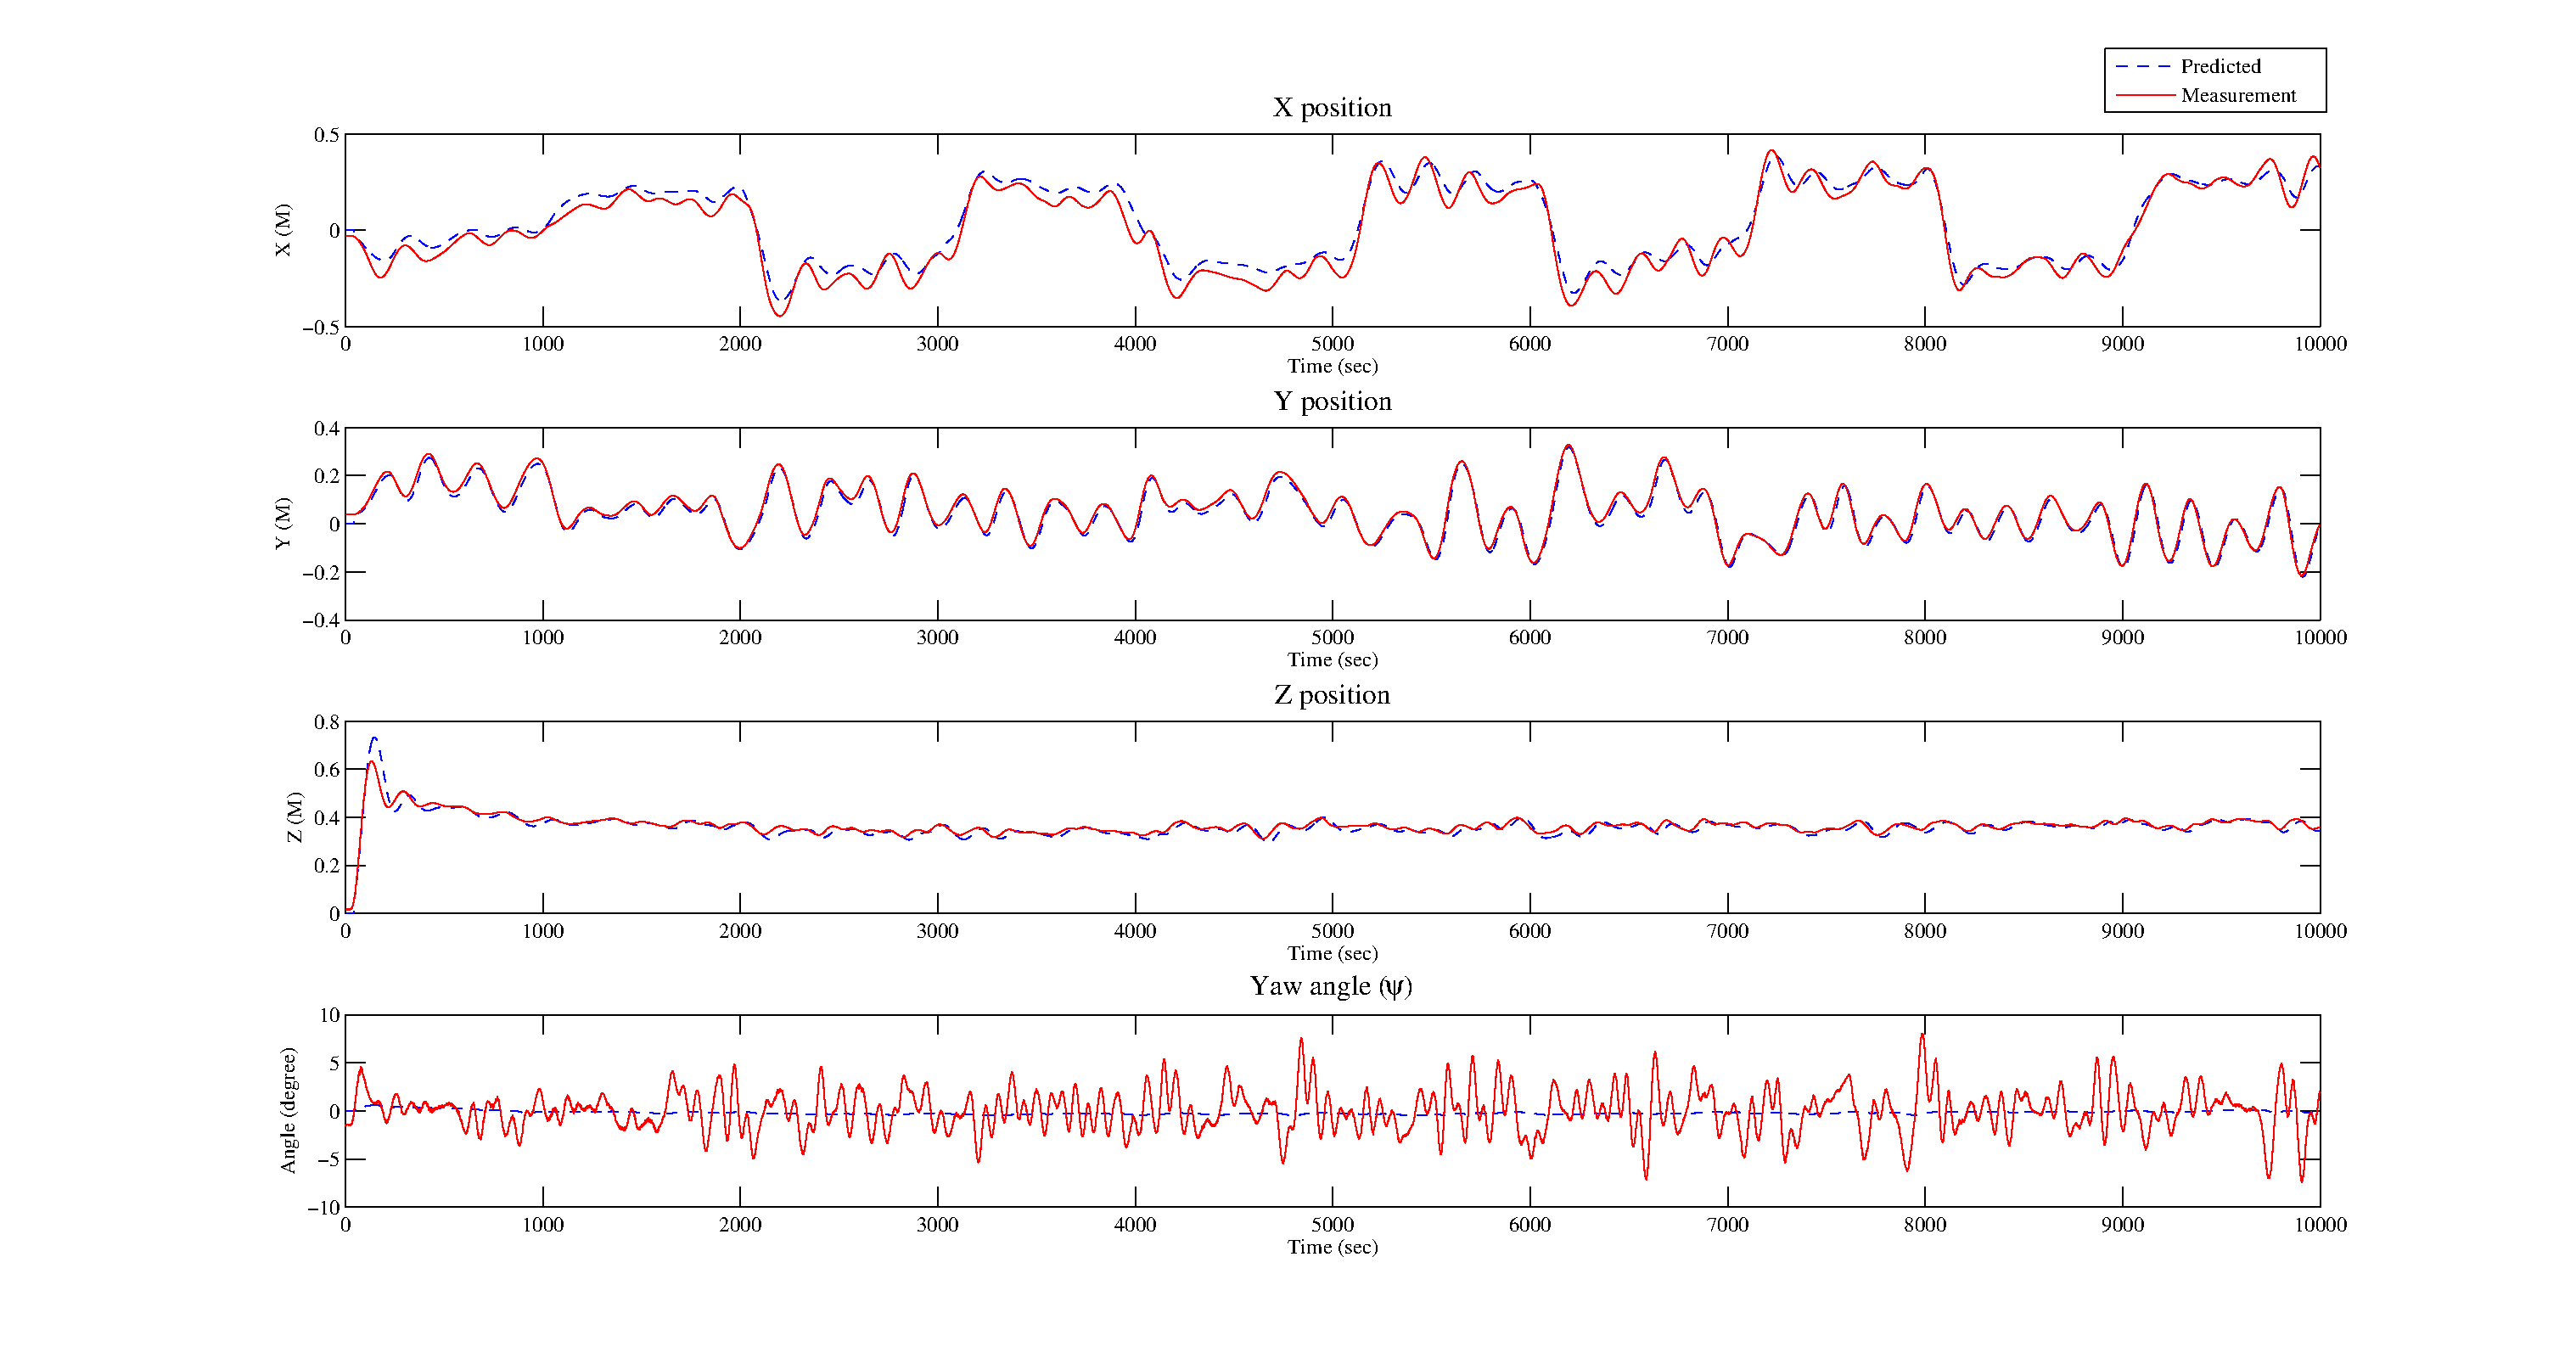
\includegraphics[width=\textwidth]{part1_xyz.eps}
	 	\caption{The result of Robot Position and orientation, separately.}
	 \end{center}
 \end{figure}

\noindent \textbf{Part 2} Find the best value for the parameter $c_0$\\
In part 1, $c$ is a constant related to thrust, here I will use following equation to compute $c$:
\begin{equation}
	c= (0.000409s^2+0.1405s-0.099)/c_0\;where s=255/600\times (thrust)
\end{equation}
In part 2, I change the values of $c_0$ (from $0.01$ to $1.0e+11$) and compute the average of residual (using 
equation (17) ) to find out where I can get the minimum average residual, as in figure 3.
\begin{equation}
	S(c_0)=\frac{1}{N}\sum\limits_{i = 1}^N {(x_m(k)-x^-(k))^2+(y_m(k)-y^-(k))^2+(z_m(k)-z^-(k))^2} 
\end{equation} 
  \begin{figure}[H]
	 \begin{center}
	 	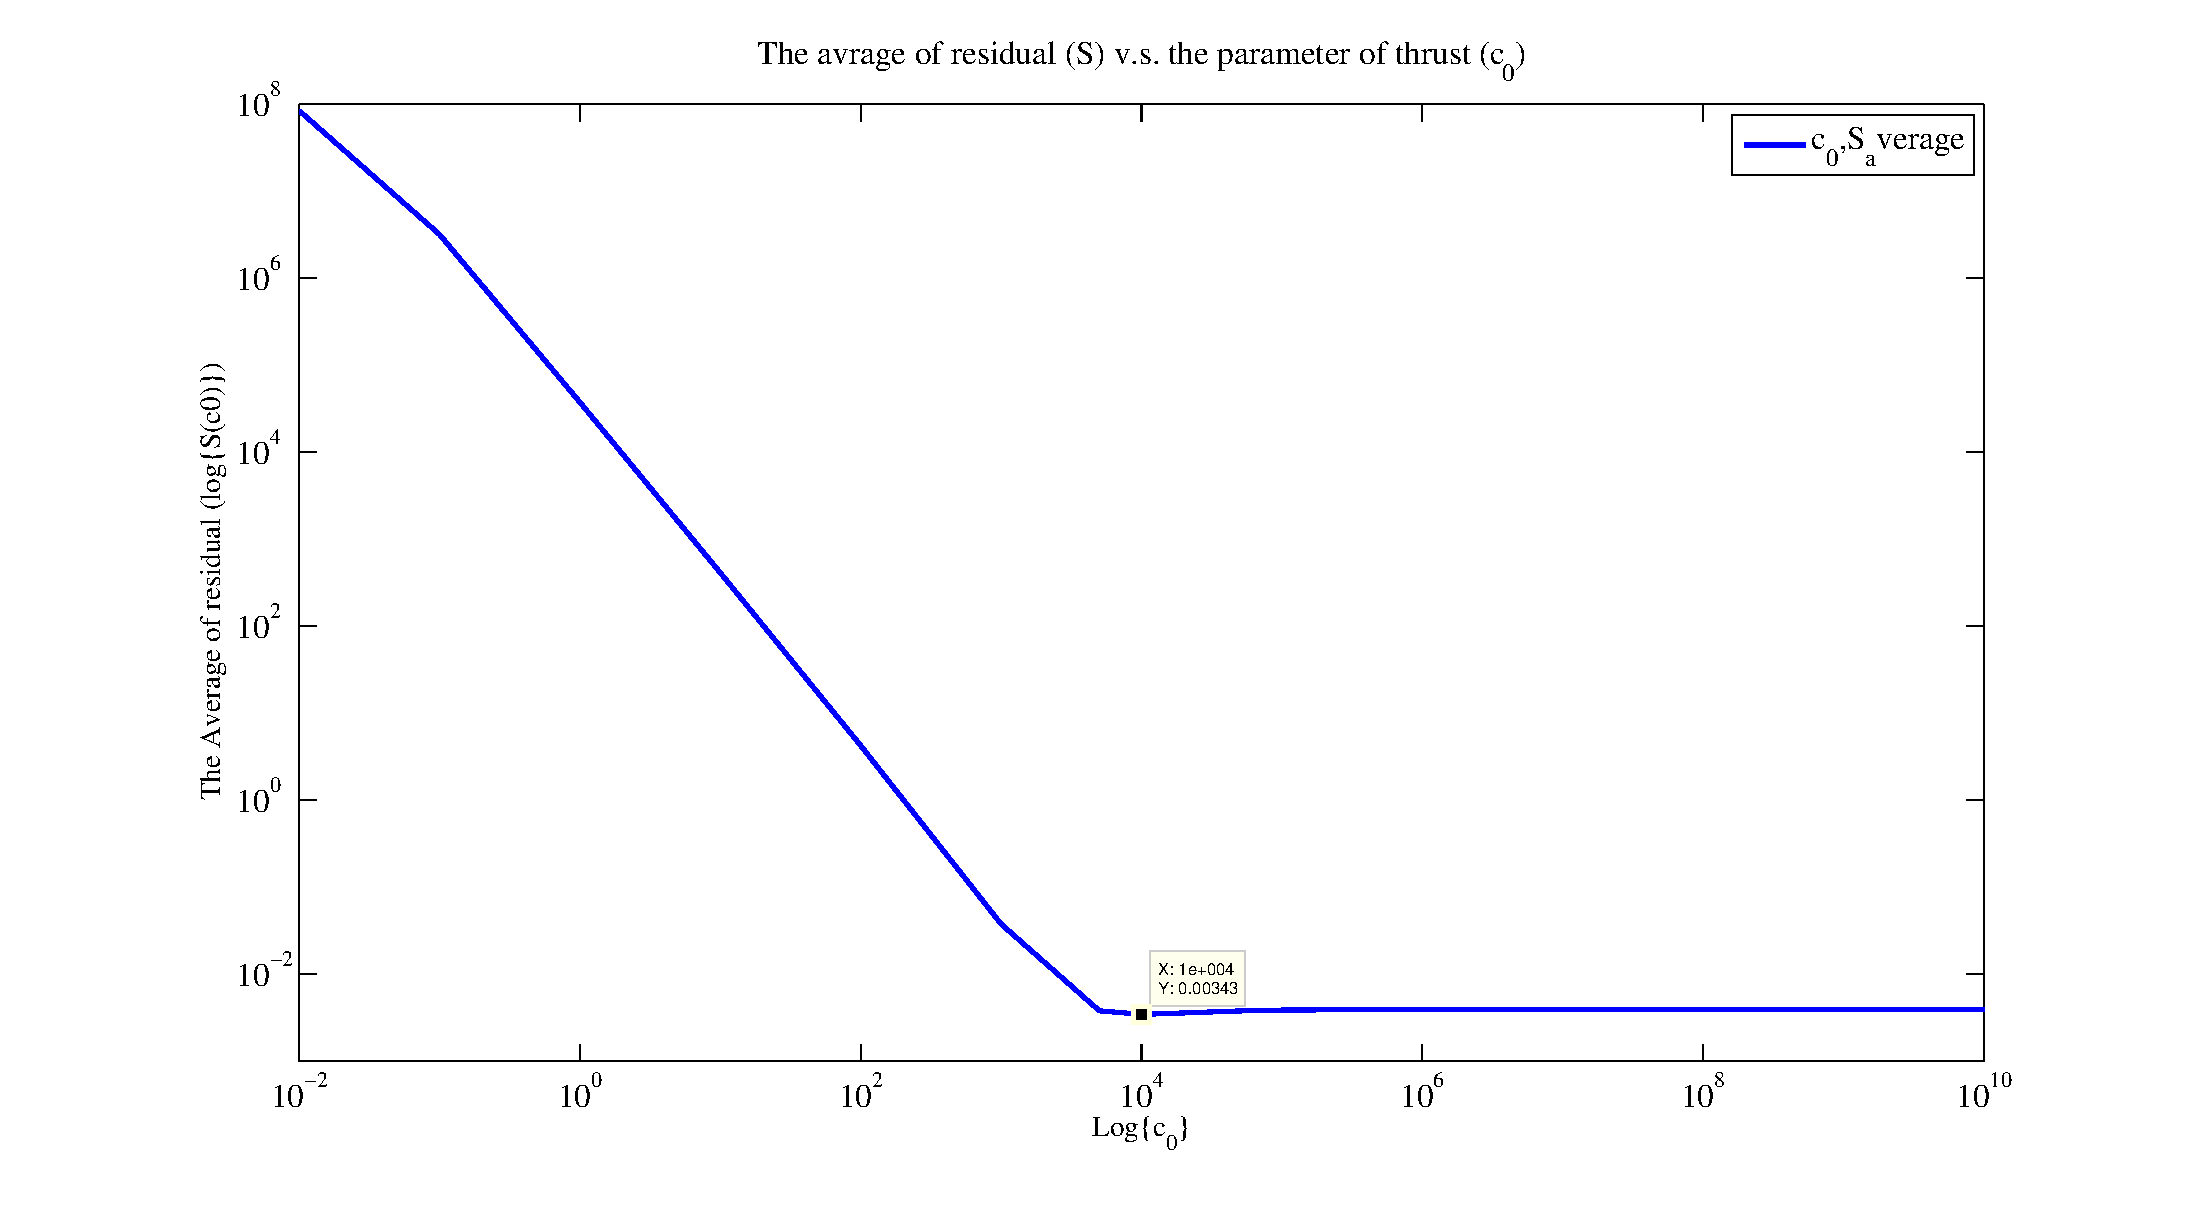
\includegraphics[width=\textwidth]{S_c0.eps}
	 	\caption{The average residual  v.s. the parameter of thrust.}
	 \end{center}
 \end{figure}
From the result of figure 3, when the parameter $c_0=10000$ (the best value), the extended Kalman filter will 
have the minimum average residual ($S(c_0) = 0.00343$)\\
\noindent \textbf{Part 3} Deal with corrupt data with considering only x-y dynamics.\\
In part 3, because we only consider x-y dynamics, I will redesign my extended Kalman filter by remove 
parameter which is related to $z$ and $\dot{z}$. Therefore, $\Phi$ is reduced to $5\times5$ matrix and 
$\Gamma$ is reduced to $5\times3$ matrix. Next, because there are corrupted data of yaw angle in the given 
measurement data, I will use the same method in part 2 to get the average residual ($498.16$). Then, when 
compute the residual in the loop of Kalman filter, I will ignore the difference of yaw angle if the original residual 
is bigger than $498.16$. 

  \begin{figure}[H]
	 \begin{center}
	 	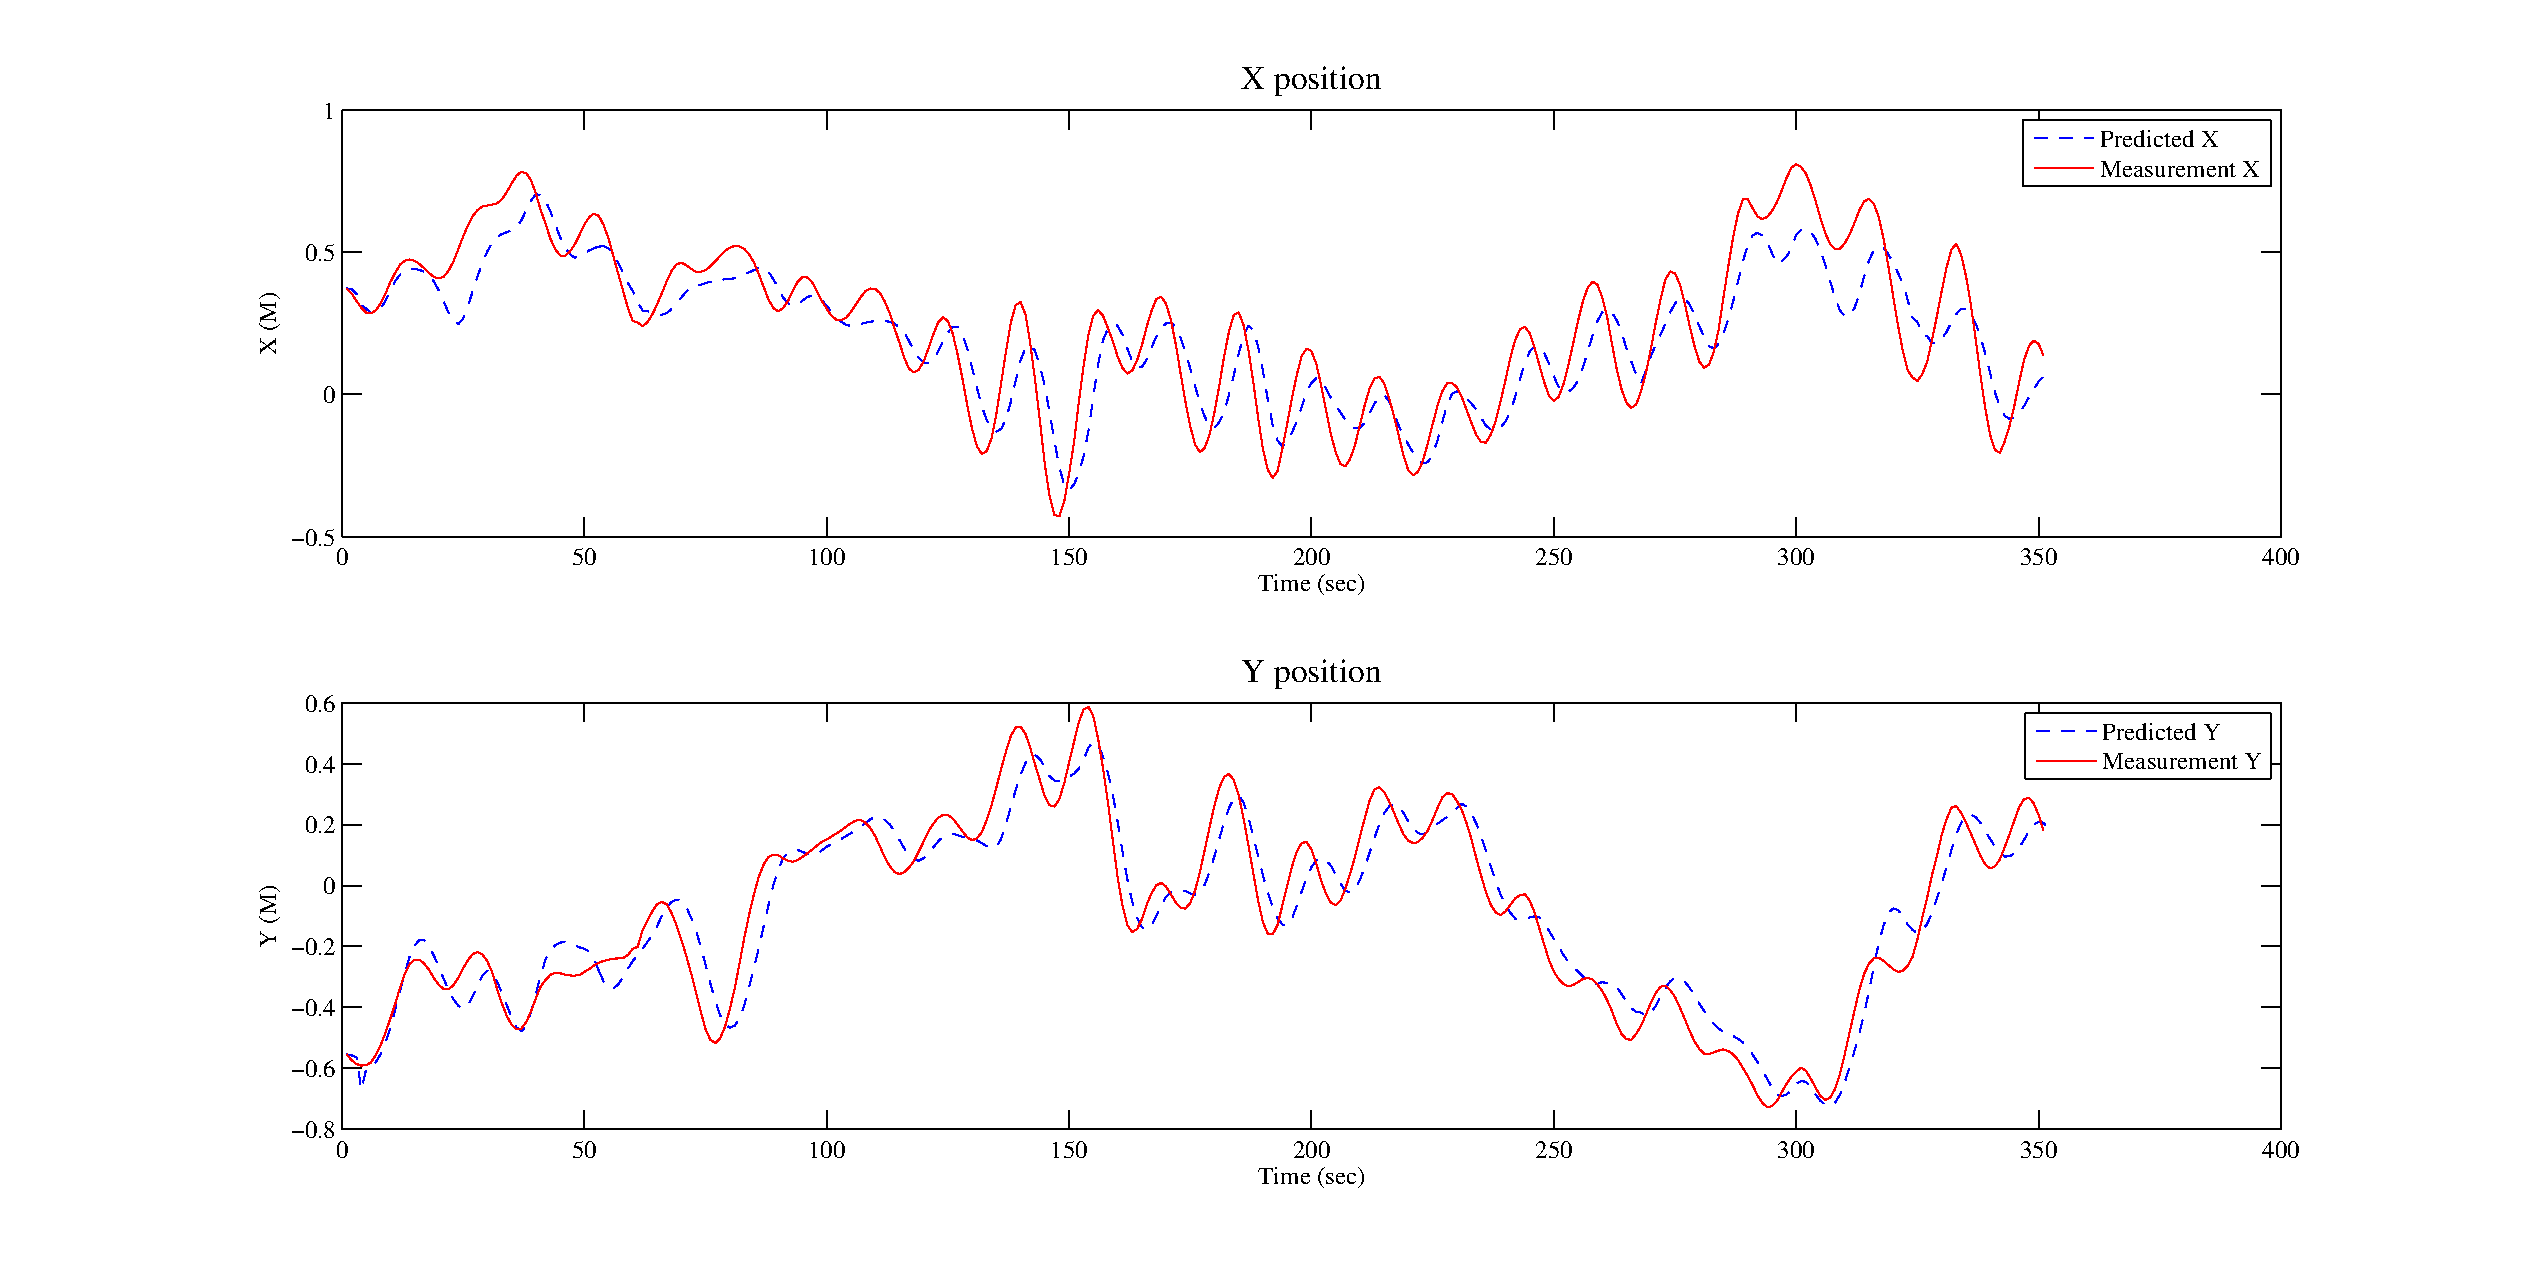
\includegraphics[width=\textwidth]{part3_xy.eps}
	 	\caption{The result of Robot Position (x-y coordination).}
	 \end{center}
 \end{figure}
 From the result of figure 4, the expected robot position (x, y) are smooth and converge with the 
 measurement data. Furthermore, in figure 5, the expected yaw angle is more smooth (with slightly shift) and 
 follow the changing of the measurement yaw angle, and Kalman filter is able to detect those corrupted data 
 from the given measurement data.
 \begin{figure}[H]
	 \begin{center}
	 	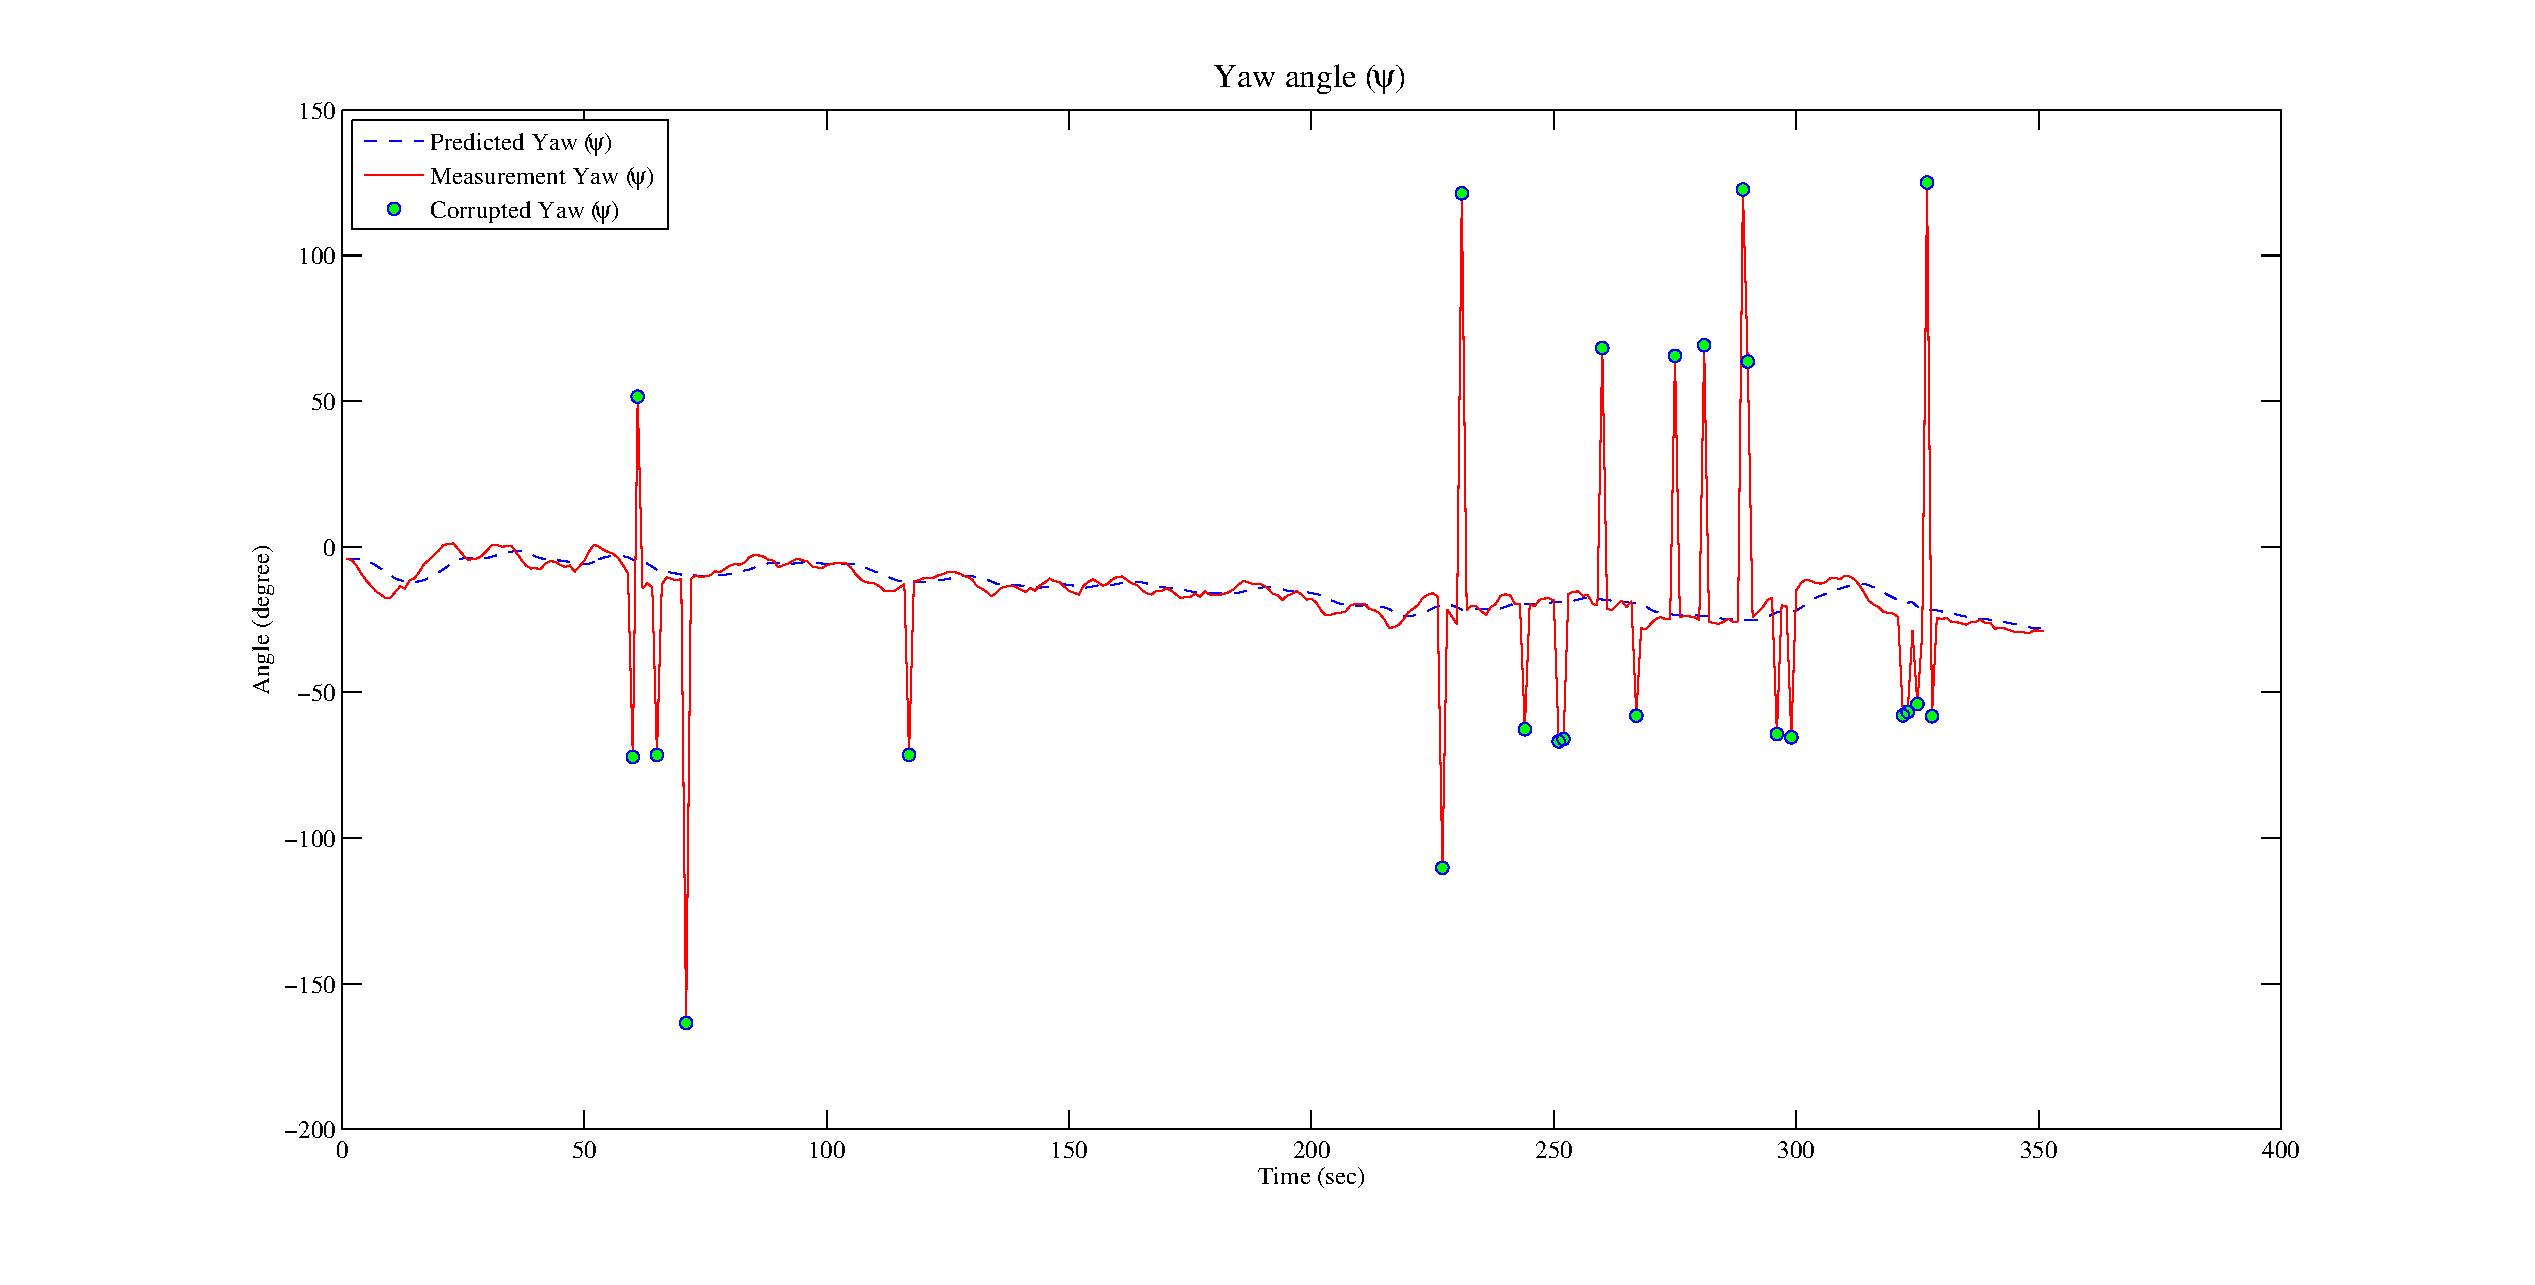
\includegraphics[width=\textwidth]{part3_yaw.eps}
	 	\caption{The result of yaw angle with corrupted data.}
	 \end{center}
 \end{figure}

\end{document}